\section{Results}
\subsection{Vegetation classification}
The vegetation classification resulted in a map showing three different classes (figure \ref{fig:classification}): points removed during preprocessing (e.g. low-stature vegetation, bare soil, water bodies), points classified as non-tall-vegetation structures (e.g. building edges, ditches and railroad infrastructure) and points belonging to tall vegetation. The accuracy assessment of this classification showed a producer's accuracy of 0.98 for \textit{vegetation} and of 0.85 for \textit{other}. The AUROCC of 0.98 showed that the \textit{vegetation} and \textit{other} class were well separated, and this was also supported by an MCC value of 0.76 (indicating of a positive correlation between the predicted and observed classes) and the geometric mean of 0.90.

\begin{figure}
	\centering
	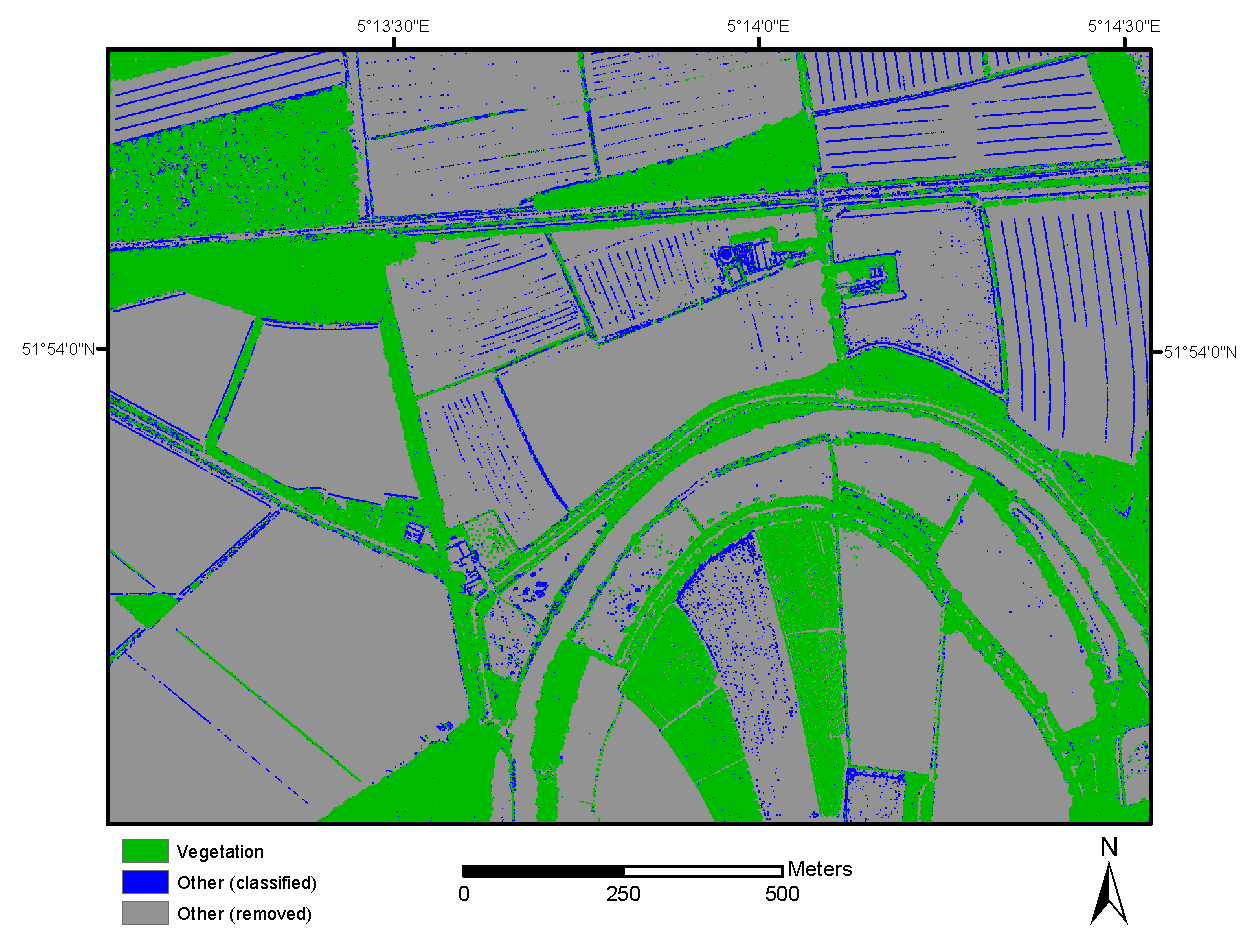
\includegraphics[width=\columnwidth]{./img/classification.pdf}
	\caption{Results of the vegetation classification. Grey areas represent data points which were removed during the preprocessing (e.g. grasslands, agricultural fields, bare soil, water bodies). Blue represents points which were not removed during the preprocessing, but classified as \textit{other} (mainly building edges, ditches and railroad infrastructure). Green represents points which were not removed during the preprocessing, but classified as tall vegetation.}
	\label{fig:classification}
\end{figure}

\begin{table}
	\caption{A confusion matrix showing the predicted classes against the actual classes of the points. These are accumulated over the 10 fold cross-validation.}
	\label{tab:confmatclass}
	\begin{tabular}{l l l l l l l}
		\toprule
		& & & \multicolumn{2}{c}{\textbf{Predicted}} & & \\
		& & & Vegetation & Other & & \\
		\midrule
		\parbox[t]{2mm}{\multirow{4}{*}{\rotatebox[origin=c]{90}{\textbf{Actual}}}} & & & & & & \\
		& Vegetation & & 974177 & 22908 & & \\
		& Other & & 8171 & 47999 & & \\
		& & & & & & \\
		\bottomrule
	\end{tabular}
\end{table}

\subsection{Linear object segmentation}
The vegetation was segmented using a region growing algorithm, the resulting objects were filtered for linearity and the results were compared with the manual segmentation (figure \ref{fig:segmentation}). This resulted in areas that were correctly classified as linear vegetation elements (true positives) and the regions that were accurately classified as nonlinear vegetation objects (true negatives). Some nonlinear areas were misclassified as linear (false positives), and some linear regions were classified as nonlinear (false negatives). However, the confusion matrix (table \ref{tab:confmatseg}) showed an overall good accuracy of 0.90, an F1-score of 0.82, and an MCC of 0.76. Hence, the majority of linear vegetation elements were successfully segmented, with user's and producer's accuracies of 0.85 and 0.80, respectively. Non-linear objects were successfully separated well, with user's and producer's accuracies of 0.92 and 0.94, respectively.

\begin{figure}
	\centering
	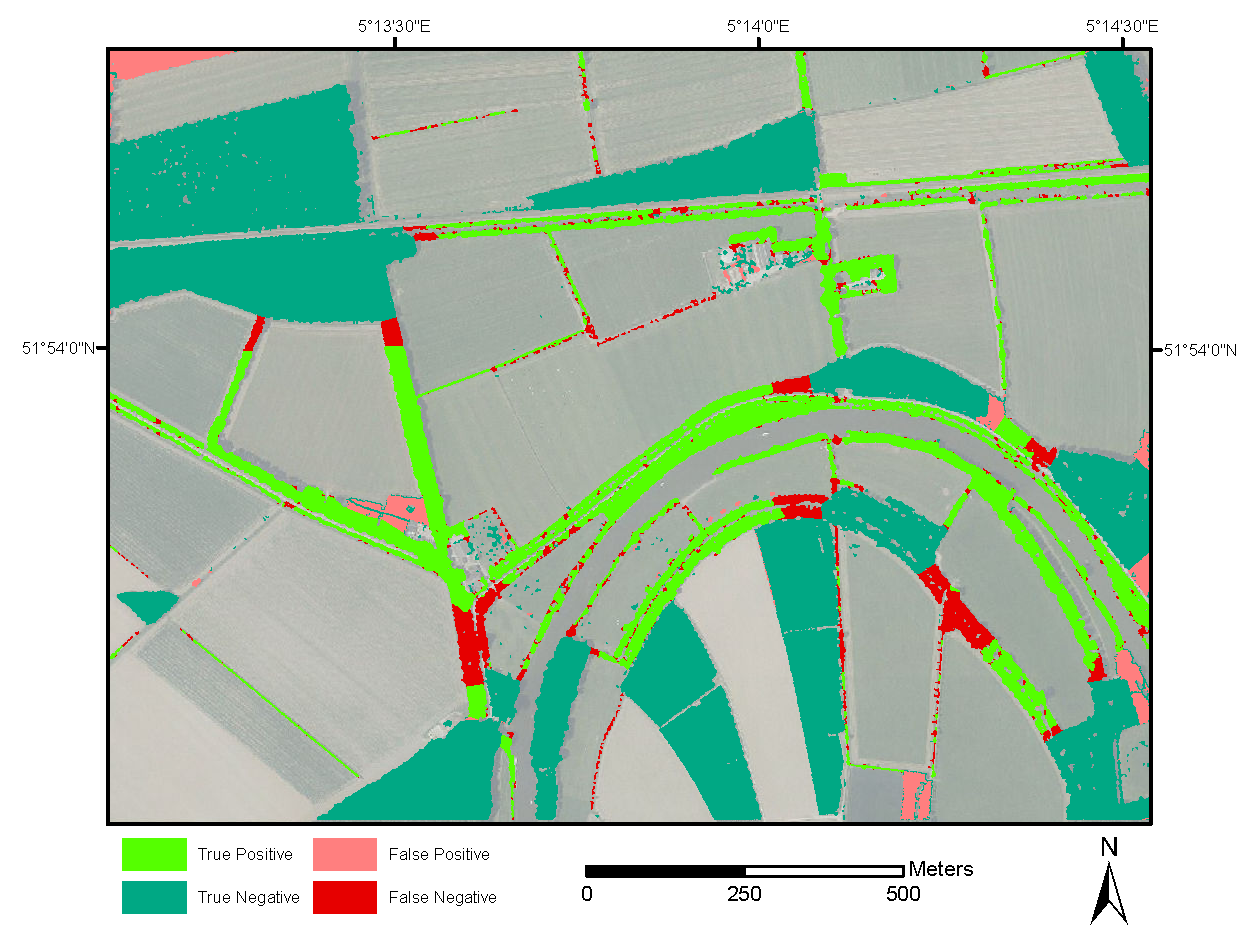
\includegraphics[width=\columnwidth]{./img/segmentation.pdf}
	\caption{Results of the segmentation of linear elements. The correctly delineated areas are shown in green, where true positive (light green) means correctly classified as a linear element and true negative (dark green) as a nonlinear element. The misclassified areas are shown in red, where false positive (light red) means classified as a linear elements, while actually being a nonlinear element, and false negative (dark red) classified as a nonlinear object, while actually being a linear.}
	\label{fig:segmentation}
\end{figure}

%\begin{table}
%	\caption{Confusion matrix listing the automatically segmented against the manually annotated set of linear and non-linear vegetation objects in area (\(m^{2}\)).}
%	\label{tab:confmatseg}
%	\begin{tabular}{l l l l l l l l}
%		\toprule
%		& & & \multicolumn{2}{c}{\textbf{Predicted}} & & & \\
%		& & & Linear & Nonlinear & & Producer's accuracy & \\
%		\midrule
%		\parbox[t]{2mm}{\multirow{4}{*}{\rotatebox[origin=c]{90}{\textbf{Actual}}}} & & & & & & & \\
%		& Linear & & 1159762 & 23438 & & & \\
%		& Nonlinear & & 6416 & 16706 & & & \\
%		& & & & & & & \\
%		& User's accuracy & & & & & & \\
%		\bottomrule
%	\end{tabular}
%\end{table}

\begin{table}
	\caption{Confusion matrix listing the automatically segmented against the manually annotated set of linear and non-linear vegetation objects in area (\(m^{2}\)).}
	\label{tab:confmatseg}
	\begin{tabular}{l l l l l l l}
		\toprule
		& & & \multicolumn{2}{c}{\textbf{Predicted}} & & \\
		& & & Linear & Nonlinear & & \\
		\midrule
		\parbox[t]{2mm}{\multirow{4}{*}{\rotatebox[origin=c]{90}{\textbf{Actual}}}} & & & & & & \\
		& Linear & & 116483.76 & 28385.56 & & \\
		& Nonlinear & & 20201.53 & 336754.65 & & \\
		& & & & & & \\
		\bottomrule
	\end{tabular}
\end{table}